The goal of land cover mapping is to make a classification of different areas the Earth's global surface. Since land cover classification has several economical/social applications, such as, monitoring and environmental planning, it is crucial that classification maps be generated with high accuracy.

Classification maps can be generated in two different ways: by field measuring or through remote sensing. Field measuring provides a high accuracy classification map but there is the obvious problem that it does not scale well to large cover areas, since it takes a lot of time, money and it is limited to areas that can be easily accessed. 

Because of these problems mentioned above, classification maps are normally generated by using remote sensing data. The GlobCover (European Space Agency GlobCover Portal) map is one example of a classification map that was generated using MERIS data.

Some of the different areas of interest can be classified as: Vegetated areas, artificial surfaces (human made surfaces like constructions, buildings, roads, houses, etc...), water bodies, permanent snow or ice, among others. Some of these classes can be subclassified among different classes, for example, vegetation can mean: irrigated croplands, deciduous forests, mosaic grassland among others. The GlobCover classification map, provided by the European Space Agency is used to perform classification (European Space Agency GlobCover Portal). The GlobCover is composed of 23 different classes, which can be seen in the figure below. 

\begin{figure}[H]
    \centering
    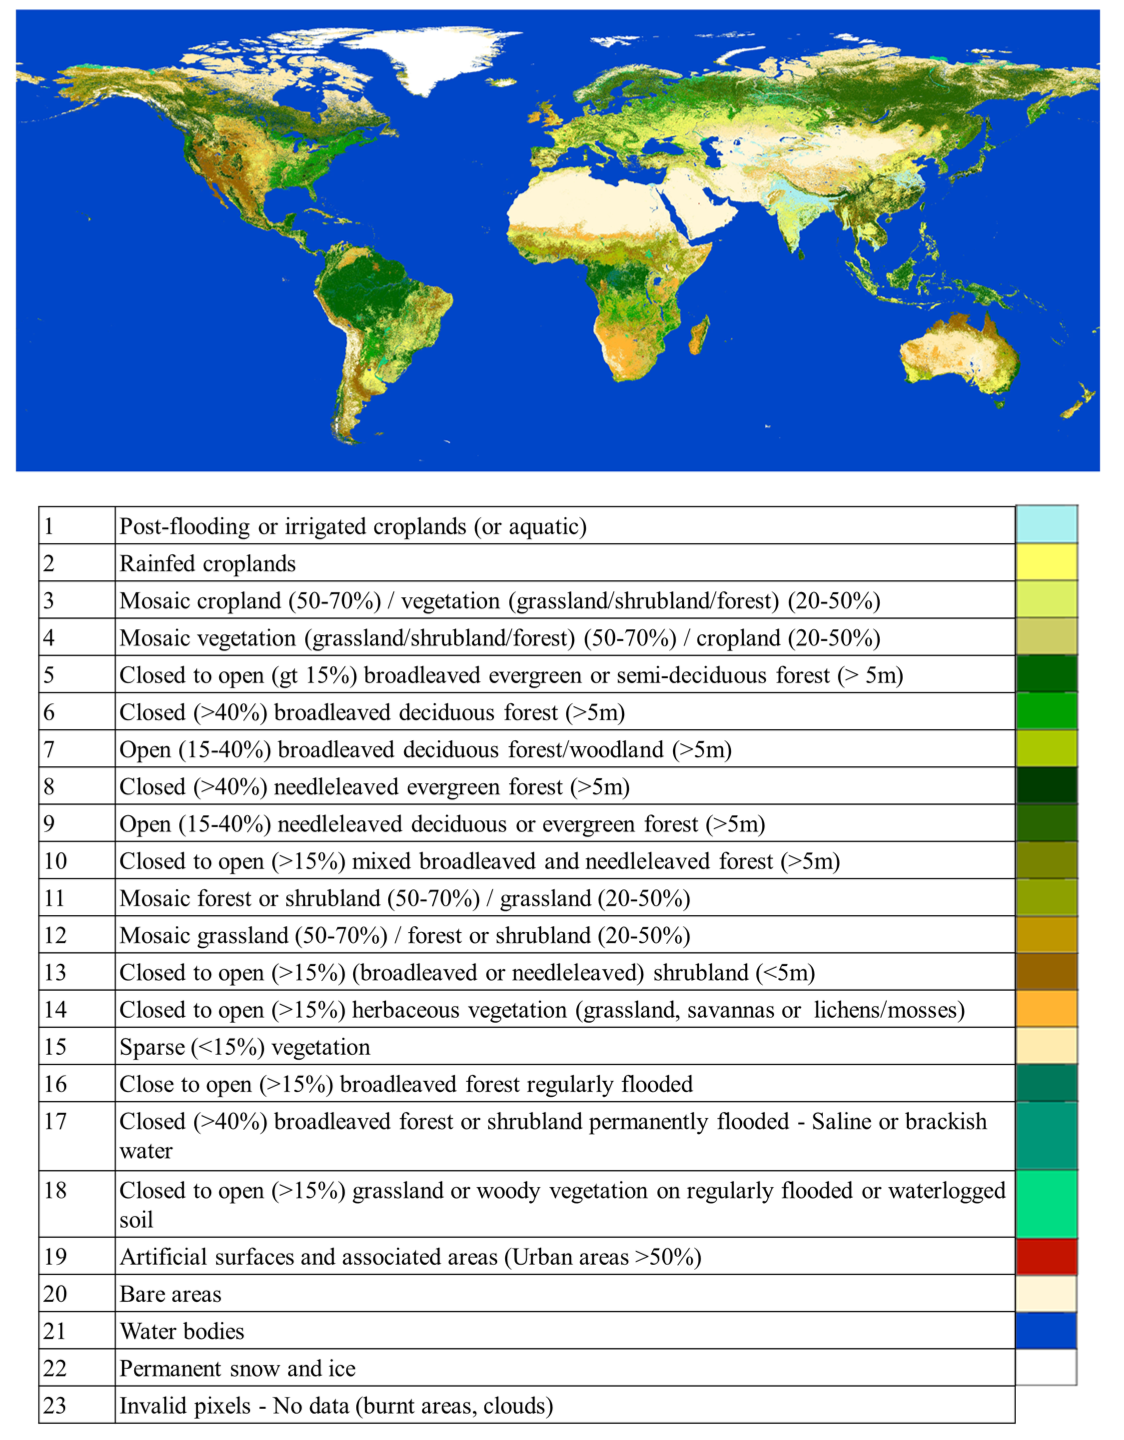
\includegraphics[width=\linewidth]{Cap2/glob_cover.png}
    \caption{GlobCover classification map.}
    \label{fig:glob_cover_map}
\end{figure}

Among the different classes mentioned above forests are a class that plays a key role in Earth's ecosystem. Therefore it is very important to analise the deforestation or change in forest areas in order to assess the impact of the ecosystem. 

Nowadays, optical and lasers sensors are used for land cover classification and forest changes, each with its own advantages. For example, optical sensors provide an easy way to make classification, but it has the disadvantages that it is weather dependent and cannot provide a high resolution map. SAR mapping has none of these disadvantages but it is harder to make a accurate classification. Given the necessity to generate classification maps throughout the year, independent of cloud coverage, detected SAR backscatter is widely used for forest mapping \cite{Krieger}. 

Some of these maps are very successful in the task of making an accurate forest map, such as the gobal forest/nonforest map L-Band ALOS PALSAR which was generated creating a threshold on the cross-polarization levels of the detected backscatter. Even though it is possible to generate classification maps using the signature backscatter, this work will focus on the creation of said maps by analizing the interferometric coherence.

The first use of interferometric data for forest mapping is reported on \cite{first_interferometric}. This work was used using ERS-1 SAR data and not only proved that forests can be clearly discriminated from other land categories, but it also showed that it is possible to distinguish among different forests types. This first approach consisted of analyzing the different values for the mean and standard deviation of the coherence for different areas, and by verifying that these values are separated. This method is visually explained in \figref{fig:first_interferometric_estimate}.

\begin{figure}[H]
    \centering
    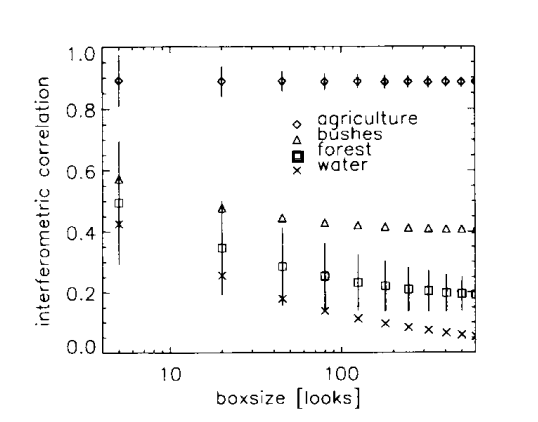
\includegraphics[width=0.7\linewidth]{Cap2/first_interferometric.png}
    \caption{Mean and Standard deviation of the coherence estimate as number of looks (filter size) for different classes.}
    \label{fig:first_interferometric_estimate}
\end{figure}

Nowadays, interferometric data can be used to monitor not only deforestation, but a series of other phenomena like topographical change and ice melting on polar caps \cite{Paolathesis}. 

On this work it will be presented the use of the ESA Sentinel-1 mission and its applications for forest mapping using the interferometric acquired data.

The Sentinel-1 mission consists of two sattelites which acquire data on a small temporal baselines (normally between 6 and 12 days) which use the C-band frequency range to acquire data in swaths of over 250km in range direction. Even though, like every SAR, the main product is the backscatter received from the target, the focus of this work is to rely only on the interferometric information for classification purposes. 

Some works rely on acquiring the backscatter data over large periods of time (months or years), and then classifying the target area based on the temporal change of it \cite{long_time_series}, this method is named long-time-series classification. Since the coherence is subjected to more variation over small periods of time, it is possible to make a classification based on its value, which don't have to be acquired over months, but over a few weeks is enough, this is why this method is called short-time-series classification, and since it has the capability of generate more updated maps, it was chosen as the method for this analysis. 

On this work it will be demonstrated that the short time series interferometric information is valuable resource for classification. Besides using the temporal model for classification, the result will also be combined with state of the art machine learning algorithms in order to even more improve the accuracy of the result obtained. 

